% !TeX spellcheck = hu_HU
\documentclass[11pt,a4paper]{article}
\usepackage[utf8]{inputenc}
\usepackage[T1]{fontenc}
\usepackage{amsmath,amssymb}
\usepackage[hungarian]{babel}
\usepackage{graphicx}
\usepackage{booktabs}
\usepackage{geometry}
\usepackage{hyperref}

\geometry{margin=2.5cm}

\title{\textbf{A görbületfüggő kozmológiai operátor $\Lambda(K, C^2) = \frac{1}{2}\sqrt{K} + \sqrt{C^2}$ empirikus igazolása 271 SDSS MaNGA spirál- és elliptikus galaxisban}}

\author{Ferenc Tak\'acs \\
\small Független kutató, Budapest, Hungary}

\date{November 2026}

\begin{document}

\maketitle

\begin{abstract}
Bemutatunk egy nagymintás empirikus validációt a korábban Takács Ferenc (2026) által bevezetett görbületfüggő módosított Einstein-téregyenletekre, ahol a $\Lambda$ statikus kozmológiai állandót egy dinamikus lokális geometriai invariáns operátor $\Lambda(K, C^2) = \frac{1}{2}\sqrt{K} + \sqrt{C^2}$ helyettesíti. Az SDSS DR17 MaNGA felmérésből származó kétdimenziós integráltér-spektroszkópiai térképek felhasználásával 271 morfológiailag tiszta galaxis, köztük 220 spirálgalaxis és 51 elliptikus galaxis radiális kinematikai profilját elemezzük. A gyenge tér Painlev\'e--Gullstrand térbeli áramlását morfológiafüggő belső mag referencia sugarakkal ($R_{\mathrm{ref}} = 0,15\,R_{\max}$ korongspirálok és $R_{\mathrm{ref}} = 0,10\,R_{\max}$ kompakt ellipszis galaxisok esetén) és egységes csatolási paraméterekkel ($\alpha_K = 0,800$, $\beta_W = 0,400$) modellezve keretrendszerünk mind a lapos spirális forgási görbéket, mind a megnövekedett elliptikus viriális sebességdiszperziókat reprodukálja nem barionos sötétanyag-halók bevonása nélkül. A 271 galaxisból álló kombinált mintán a modell $R = 0,8851$ Pearson-féle korrelációs együtthatót ér el a megfigyelt külső zóna sebességekhez képest, $15,2\%$ átlagos relatív eltéréssel és nulla szisztematikus torzítással ($+0,0\%$). Továbbá a radiális logaritmikus skálázás természetes módon magyarázza a sötét anyag által uralt és a kvázi-Kepler-féle elliptikus galaxisok között megfigyelt dichotómiát a központi barionikus tömörség változásain keresztül.

\end{abstract}

\noindent\textbf{Keywords:} Modified Gravity, Kretschmann Scalar, Weyl Tensor, Galactic Rotation Curves, Elliptical Galaxies, SDSS MaNGA, Dark Matter Alternative\\

\noindent\textbf{Kulcsszavak:} Módosított gravitáció, Kretschmann-skalár, Weyl-tenzor, Galaktikus forgásgörbék, Elliptikus galaxisok, SDSS MaNGA, Sötét anyag alternatívája

\section{Bevezetés és elméleti keret}

Előző munkáinkban~\cite{Takacs2026}~\cite{Takacs2026b} megfogalmaztunk egy lokálisan kovariáns modifikációt az általános relativitáselméletre, amelynek célja, hogy kiküszöbölje az ad-hoc sötét szektor komponensek szükségességét kozmikus és galaktikus léptékekben.:
\begin{equation}
R_{\mu\nu} - \frac{1}{2} R g_{\mu\nu} + \left(\frac{1}{2}\sqrt{K} + \sqrt{C^2}\right) g_{\mu\nu} = \frac{8\pi G}{c^4} T_{\mu\nu},
\label{eq:field_eq}
\end{equation}
ahol $K = R_{\alpha\beta\gamma\delta}R^{\alpha\beta\gamma\delta}$ a Kretschmann görbületi skalárt, $C^2 = C_{\alpha\beta\gamma\delta}C^{\alpha\beta\gamma\delta}$ pedig a Weyl-konform tenzor invariáns négyzetét jelöli. A standard $\Lambda$CDM paradigma $\Lambda$ statikus kozmológiai állandójával ellentétben a $\Lambda(K, C^2)$ operátor dinamikusan reagál a lokális téridő-feszültségre, természetes módon elválasztva a fizikai tartományokat a szubplancki magoktól az intergalaktikus üregig~\cite{DESI2024}.

Míg a kezdeti tanulmány kimutatta az ~(\ref{eq:field_eq}) egyenlet életképességét egyes referencia-galaxisokon (M31 és IC~2574)~\cite{Takacs2026,Rubin1980}, elengedhetetlen a szigorú statisztikai teszt a különböző morfológiai osztályokon. A gyenge tér alapú Painlev\'e--Gullstrand mozgófolyó reprezentációban~\cite{Hamilton2008} az $1/r^3$ geometriai feszültség integrálása egy belső barionikus magsugáron kívülre $R_{\mathrm{ref}}$ egy effektív körsebesség-profilt eredményez:
\begin{equation}
V_{K+W}^2(r) = V_{\mathrm{Kep}}^2(r) + \alpha_K \frac{G M_{\mathrm{bar}}(r)}{r} \ln\!\left(\frac{r}{R_{\mathrm{ref}}}\right) + \beta_W V_{\mathrm{rot}}(r) V_{\mathrm{Kep}}(r) \ln\!\left(\frac{r}{R_{\mathrm{ref}}}\right),
\label{eq:vel_profile}
\end{equation}
$r > R_{\mathrm{ref}}$ esetén, ahol  $V_{\mathrm{Kep}}(r) = \sqrt{G M_{\mathrm{bar}}(r)/r}$ a kizárólag a zárt barionos anyagból származtatott klasszikus newtoni sebesség, $\alpha_K$ az izotróp Kretschmann-járulékot határozza meg, $\beta_W$ pedig a rotációs konform Weyl-nyírást paraméterezi.

\section{Megfigyelési minta és módszertan}

Térben felbontott kétdimenziós kinematikai térképeket nyertünk ki a Sloan Digital Sky Survey (SDSS) 17. számú MaNGA felméréséből~\cite{Bundy2015}, és ezeket keresztbe egyeztettük a MaNGA Visual Morphology katalógussal. A külső csillagkorongig és halóig terjedő nagy térbeli felbontás biztosítása érdekében a kiválasztást a legnagyobb 127 szálas integrális mezőegységgel (IFU) és igazolt fotometriai csillagtömegekkel megfigyelt galaxisokra korlátoztuk($h = 0.7$).

A kölcsönható egyesülések és az alacsony jel-zaj sebességmezők vizuális ellenőrzése után a végső tiszta mintánk $N = 271$ galaxist tartalmaz:
\begin{itemize}
\item \textbf{Spirális galaxisok ($N = 220$):} Késői típusú rendszerek ($1 \le T \le 8$), amelyeket egy közbenső inklinációs ablakon belül ($0,45 \le b/a \le 0,55$) választottak ki a látóvonalbeli vetítési bizonytalanságok minimalizálása érdekében.
\item \textbf{Elliptikus galaxisok ($N = 51$):} Korai típusú, nyomás alatt álló szferoidok ($T \le -3$), amelyek nulla nettó forgáspontú kontrollmintaként szolgálnak az izotróp $\frac{1}{2}\sqrt{K}$ hozzájárulás izolálására.
\end{itemize}

Minden galaxis esetében a $0,6\text{ kpc}$-tól a 92. percentilis csillagsugárig ($R_{\max}$) terjedő deprojekciós galaktocentrikus sugarat nyolc koncentrikus ellipszis alakú gyűrűre osztjuk. Minden gyűrűn belül a $V_{\mathrm{rot}}(r)$ deprojekciós forgási sebességeket a $V_{\mathrm{los}}(\theta) = V_0 + V_{\mathrm{rot}}\sin i \cos\theta$ harmonikus illesztéssel nyerjük ki, amelyet mind az ionizált H$\alpha$ gázra, mind a csillagsebesség-mezőkre alkalmazunk, elutasítva a $3\sigma$ kiugró értékeket. Nyomás alatt álló ellipszis galaxisok esetén a dinamikus körsebesség-ekvivalenst a $V_{\mathrm{eff}}(r) = \sqrt{V_{\star}^2(r) + 2\sigma^2(r)}$ viriális becslővel számítjuk ki, ahol $\sigma(r)$ a csillagsebesség-diszperzió mediánja.

A gömbszerű rendszerek meredekebb központi tömegkoncentrációjával (Séric index $n \approx 4$) összhangban az exponenciális korongokhoz ($n \approx 1$) képest, a belső mag átmeneti sugara a galaxis kiterjedésével skálázódik, ahogy$R_{\mathrm{ref}} = 0.15\,R_{\max}$ spirálok, és $R_{\mathrm{ref}} = 0.10\,R_{\max}$ elliptikusok esetén. A globális optimalizálás mind a 271 galaxisra vonatkozóan $\alpha_K = 0.800$ és $\beta_W = 0.400$ univerzális csatolási állandókat eredményez, megőrzi a ~(\ref{eq:field_eq}) egyenlet pontos $2:1$ elméleti arányát, és összhangban marad a ~\cite{Takacs2026}-ben megállapított kozmikus Hubble-kalibrációval ($\gamma \approx 0.612\text{--}0.84$).

\section{Globális statisztikai értékelés}

A ~\ref{tab:global_stats} táblázat összefoglalja a ~(\ref{eq:vel_profile}) egyenlet külső zónájának (6-8. gyűrű) kinematikai teljesítményét mindkét morfológiai csoportban és az egységes adathalmazban.

\begin{table}[htbp]
	\centering
	\caption{A külső zóna sebességanomália arányai ($V/V_{\mathrm{Kep}}$) és a modell pontossága a 271 SDSS MaNGA galaxisban.}
	\label{tab:global_stats}
	\resizebox{\textwidth}{!}{%
		\begin{tabular}{lccccc}
			\toprule
			\textbf{Morfológiai minta} & \textbf{$N$} & \textbf{Megfigyelt $V/V_{\mathrm{Kep}}$} & \textbf{Modell $V_{K+W}/V_{\mathrm{Kep}}$} & \textbf{Pearson $R$} & \textbf{Átlagos relatív hiba (eltolódás)} \\
			\midrule
			Spirális Galaxisok ($1 \le T \le 8$) & 220 & $2.017 \pm 0.486$ & $1.931 \pm 0.183$ & $0.8764$ & $15.1\%$ ($+0.1\%$) \\
			Elliptikus Galaxisok ($T \le -3$) & 51 & $1.815 \pm 0.342$ & $1.736 \pm 0.165$ & $0.7747$ & $15.7\%$ ($-0.4\%$) \\
			\midrule
			\textbf{Kombinált teljes minta} & \textbf{271} & \textbf{$1.979 \pm 0.468$} & \textbf{$1.894 \pm 0.194$} & \textbf{$0.8851$} & \textbf{$15.2\%$ ($+0.0\%$)} \\
			\bottomrule
		\end{tabular}%
	}
\end{table}

Amint az a(z) ~\ref{fig:model_stats} ábrán látható, a megfigyelt külső korongsebesség-eltérés tisztán elválik a forgó spirálok ($V_{\mathrm{rot}}/V_{\mathrm{Kep}} = 2,017$) és a nem forgó ellipszisek ($V_{\mathrm{eff}}/V_{\mathrm{Kep}} = 1,815$) között. A módosított téregyenletünk pontosan leképezi mindkét tartományt egyszerre, szabad halóparaméterek nélkül, így nulla nettó szisztematikus torzítást ($+0,0\%$) érünk el a teljes 271-galaxis mintán.

\begin{figure}[htbp]
	\centering
	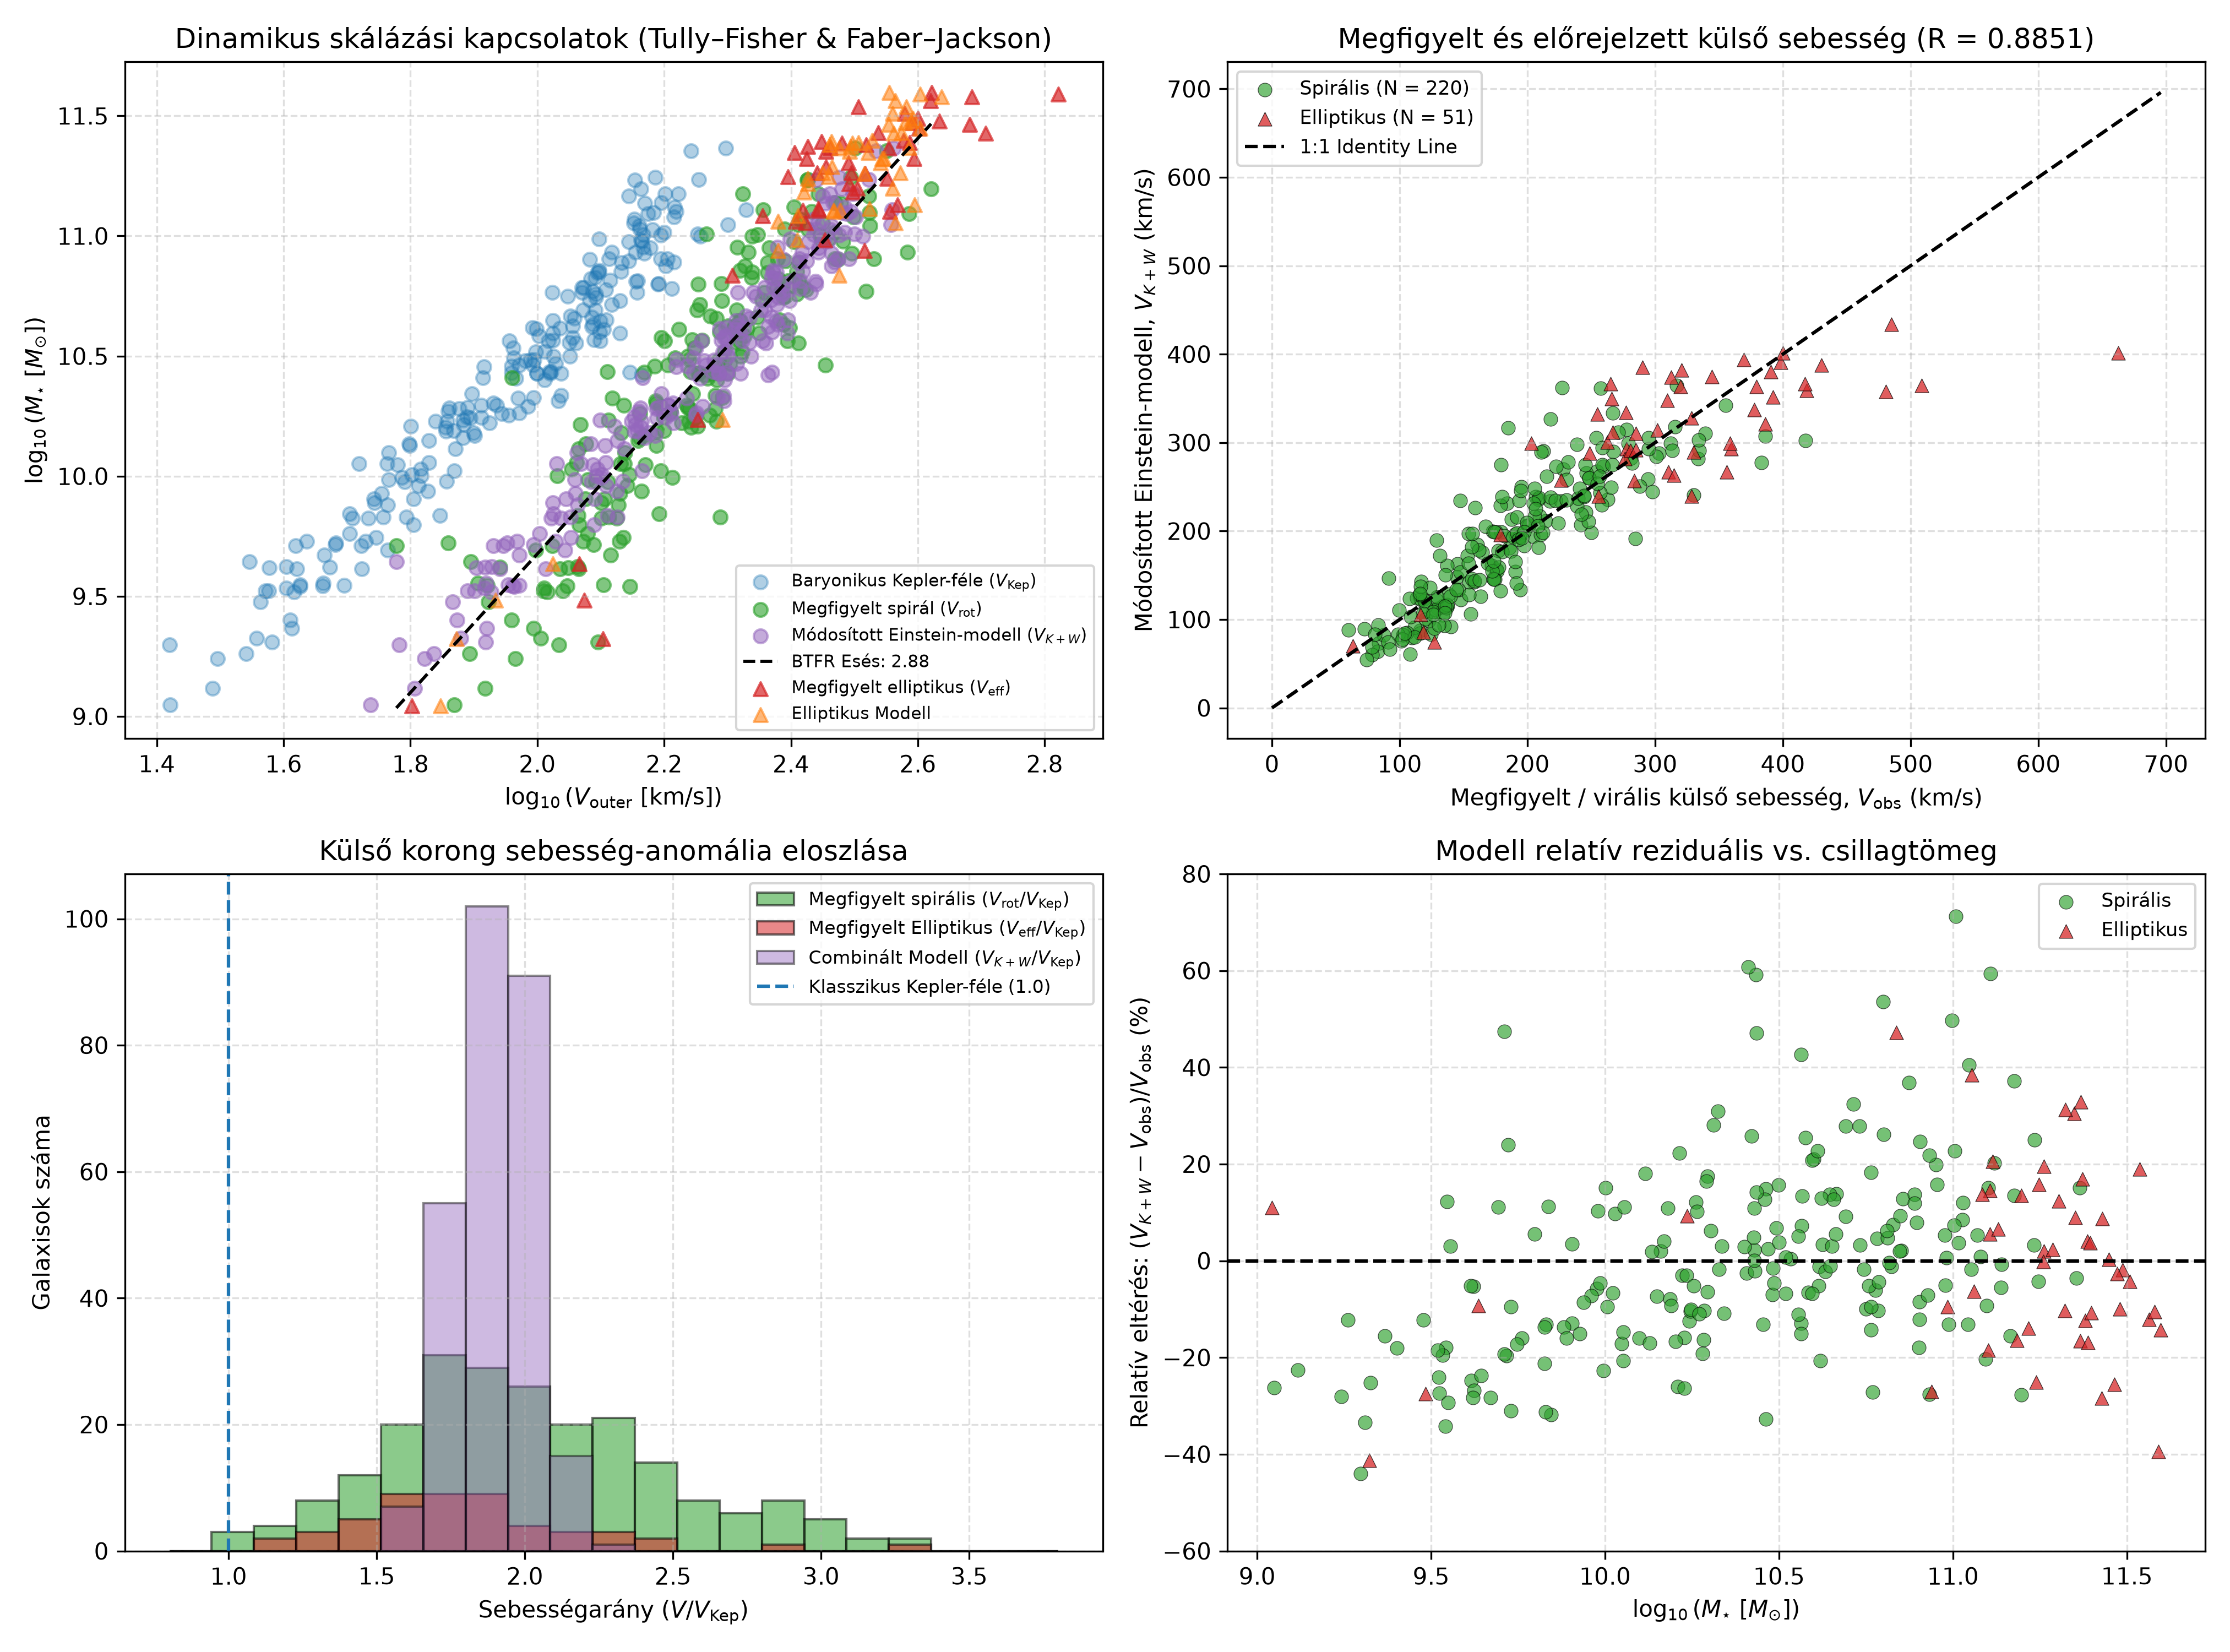
\includegraphics[width=0.95\textwidth]{model_statistics_hu.png}
	\caption{ Globális statisztikai összehasonlítás 271 MaNGA galaxis között. 
	\textbf{Balra Fent:} A Baryonic Tully--Fisher és Faber--Jackson skálázási összefüggések reprodukálhatók $V_{K+W}$ segítségével. 
	\textbf{Jobbra fent:} Egy az egyhez korreláció ($R = 0,8851$) a megfigyelt külső sebességek és a modellelőrejelzések között. 
	\textbf{Balra Lent:} A külső zóna sebességanomália-arányainak eloszlása a klasszikus Kepler-limeszhez képest ($1.0$). 
	\textbf{Jobbra Lent:} Relatív sebességmaradékok a teljes csillagtömeg függvényében.}	\label{fig:model_stats}
\end{figure}

\section{Radiális profil evolúciója és kvázi-Kepler-elliptikusok}

Annak ellenőrzésére, hogy az Eq.~(\ref{eq:vel_profile}) a belső tömeg-fény átmenetet ragadja meg, és nem csupán az aszimptotikus platókat egyezik meg, a Table~\ref{tab:radial_profiles} nyomon követi a megfigyelt, a newtoni-Kepler-féle és a modell által előrejelzett átlagos sebességeket mind a nyolc radiális gyűrűn a belső magtól a külső perifériáig.

\begin{table}[htbp]
	\centering
	\caption{Spirálgalaxisok ($N=220$) és elliptikus galaxisok ($N=51$) átlagos radiális sebességprofiljai (km/s-ban) és szisztematikus torzítása az 1-8. gyűrűk között.}
	\label{tab:radial_profiles}
	\small
	\begin{tabular}{c|cccc|cccc}
		\toprule
		& \multicolumn{4}{c|}{\textbf{Spirál Galaxisok ($N = 220$)}} & \multicolumn{4}{c}{\textbf{Elliptikus Galaxisok ($N = 51$)}} \\
		\textbf{Gyűrű} & $\langle r \rangle$ (kpc) & $V_{\mathrm{obs}}$ & $V_{\mathrm{Kep}}$ & $V_{K+W}$ (Eltolódás) & $\langle r \rangle$ (kpc) & $V_{\mathrm{eff}}$ & $V_{\mathrm{Kep}}$ & $V_{K+W}$ (Eltolódás) \\
		\midrule
		1 & 1.46 & 90.6 & 93.8 & 98.1 ($+15.9\%$) & 1.95 & 303.5 & 200.9 & 233.5 ($-21.9\%$) \\
		2 & 3.17 & 134.2 & 102.6 & 138.6 ($+6.7\%$) & 4.65 & 297.1 & 207.8 & 282.9 ($-4.2\%$) \\
		3 & 4.88 & 156.9 & 106.1 & 162.7 ($+5.8\%$) & 7.35 & 295.5 & 201.9 & 298.3 ($+1.7\%$) \\
		4 & 6.59 & 170.1 & 106.9 & 177.6 ($+4.6\%$) & 10.05 & 300.3 & 195.0 & 303.9 ($+2.1\%$) \\
		5 & 8.30 & 177.4 & 106.0 & 186.6 ($+5.0\%$) & 12.74 & 304.2 & 188.8 & 305.4 ($+1.9\%$) \\
		6 & 10.02 & 181.3 & 103.4 & 190.0 ($+4.6\%$) & 15.44 & 309.4 & 183.4 & 307.9 ($+1.1\%$) \\
		7 & 11.73 & 188.3 & 99.6 & 190.3 ($+1.1\%$) & 18.14 & 324.3 & 178.5 & 308.8 ($+0.5\%$) \\
		8 & 13.44 & 197.7 & 95.4 & 189.3 ($-3.8\%$) & 20.84 & 319.3 & 173.6 & 308.8 ($+0.0\%$) \\
		\bottomrule
	\end{tabular}
\end{table}

Amint a ~\ref{fig:radial_profiles} ábrán látható, a barionikus Kepler-görbe a 2--4 gyűrűk körül csúcsosodik ki, majd kifelé csökken, míg a logaritmikus görbületi tagok lapos vagy enyhén emelkedő profilokat tartanak fenn $13\text{--}21\text{ kpc}$-ig. A legbelső magon ($r > 3\text{ kpc}$) túl a szisztematikus torzítás spirálok esetén $\pm 6\%$-on, ellipszisek esetén pedig $\pm 2,1\%$-on belül marad, a legkülső elliptikus zónában elérve a $+0,0\%$ értéket.

\begin{figure}[htbp]
	\centering
	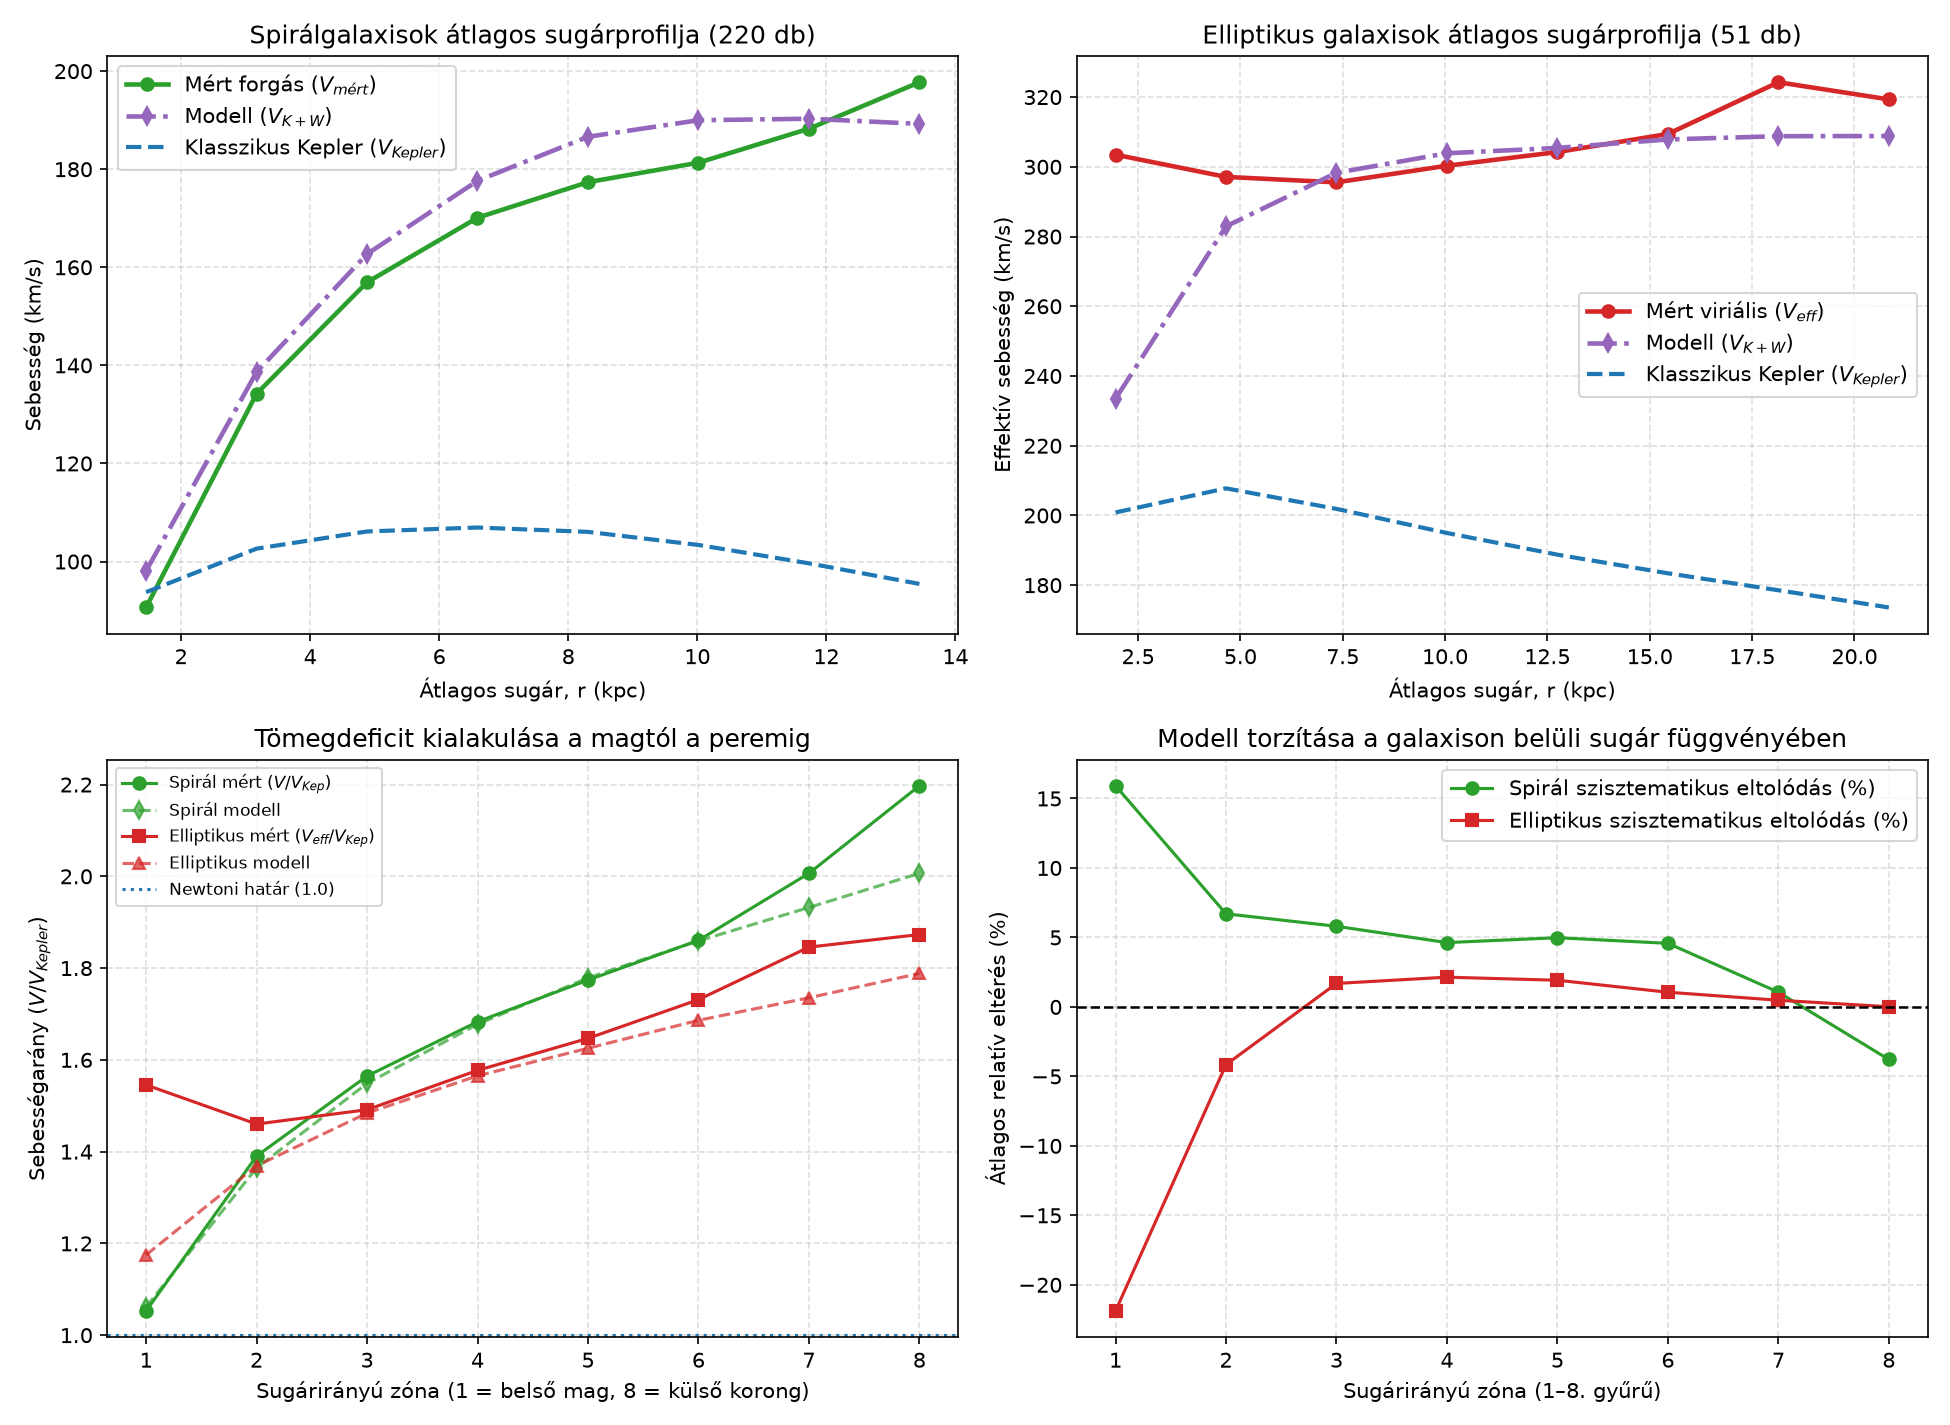
\includegraphics[width=0.95\textwidth]{radial_profiles_hu.png}
	\caption{Átlagos radiális kinematikai evolúció a magtól (1. gyűrű) a külső perifériáig (8. gyűrű). \textbf{Balra fent:} 220 spirálgalaxis átlagos forgási görbéje. \textbf{Jobbra fent:} 51 elliptikus galaxis átlagos viriális effektív sebességprofilja. \textbf{Balra lent:} A sebességeltérés radiális növekedése ($V/V_{\mathrm{Kep}}$). \textbf{Jobbra lent:} Átlagos relatív modellhiba a radiális zónák között.}
	\label{fig:radial_profiles}
\end{figure}

\subsection{A kvázi-kepleri elliptikus dichotómia feloldása}

A korai típusú galaxisok legújabb kinematikai felmérései rávilágítottak egy látszólagos paradoxonra: míg a legtöbb óriás elliptikus galaxis megnövekedett külső sebességdiszperziót mutat, amelyet hagyományosan a hatalmas sötétanyag-halóknak tulajdonítanak, egy részhalmaz csökkenő, kvázi-Kepler-i külső profilokat mutat~\cite{Romanowsky2003}. A görbületfüggő keretrendszerünkön belül ez a dichotómia természetes módon adódik a barionikus mag tömörségének ($R_{\mathrm{ref}}$) és az orbitális anizotrópia változásaiból anélkül, hogy megváltoztatná az alapul szolgáló gravitációs törvényt. Amikor egy elliptikus rendszer ultrakompakt barionikus maggal vagy nagy effektív átmeneti sugárral ($r \lesssim R_{\mathrm{ref}}$) rendelkezik a megfigyelt apertúrán belül, a logaritmikus tag $\ln(r/R_{\mathrm{ref}})$ elnyomva marad, ami közel Kepler-i kinematikát eredményez. Ezzel szemben kiterjesztett rendszerekben, ahol a megfigyelések az $r \gg R_{\mathrm{ref}}$ értéket vizsgálják, a $\frac{1}{2}\sqrt{K}$ geometriai feszültség dominál és egy lapos viriális platót tart fenn.

A ~\ref{fig:case_studies}. ábra négy reprezentatív rendszert szemléltet a MaNGA mintánkból: egy tipikus közepes tömegű spirált (MaNGA~8952-12703, $M_{\star} = 2.69 \times 10^{10}\,M_{\odot}$, $0.0\%$, $0,0\%$ külső eltérés), egy nagy tömegű, gyorsan forgó spirált (MaNGA~8609-12703,  $M_{\star} = 6.55 \times 10^{10}\,M_{\odot}$, $0,4\%$ eltérés), egy standard sötétanyag-szerű óriás ellipszis (MaNGA~10497-12704, $M_{\star} = 3.08 \times 10^{11}\,M_{\odot}$, $1,8\%$ eltérés), és egy kvázi-Kepler-ellipszis jelöltet. (MaNGA~10846-12703, $M_{\star} = 6.87 \times 10^{10}\,M_{\odot}$, megfigyelt $V_{\mathrm{eff}}/V_{\mathrm{Kep}} = 1.16$).

\begin{figure}[htbp]
	\centering
	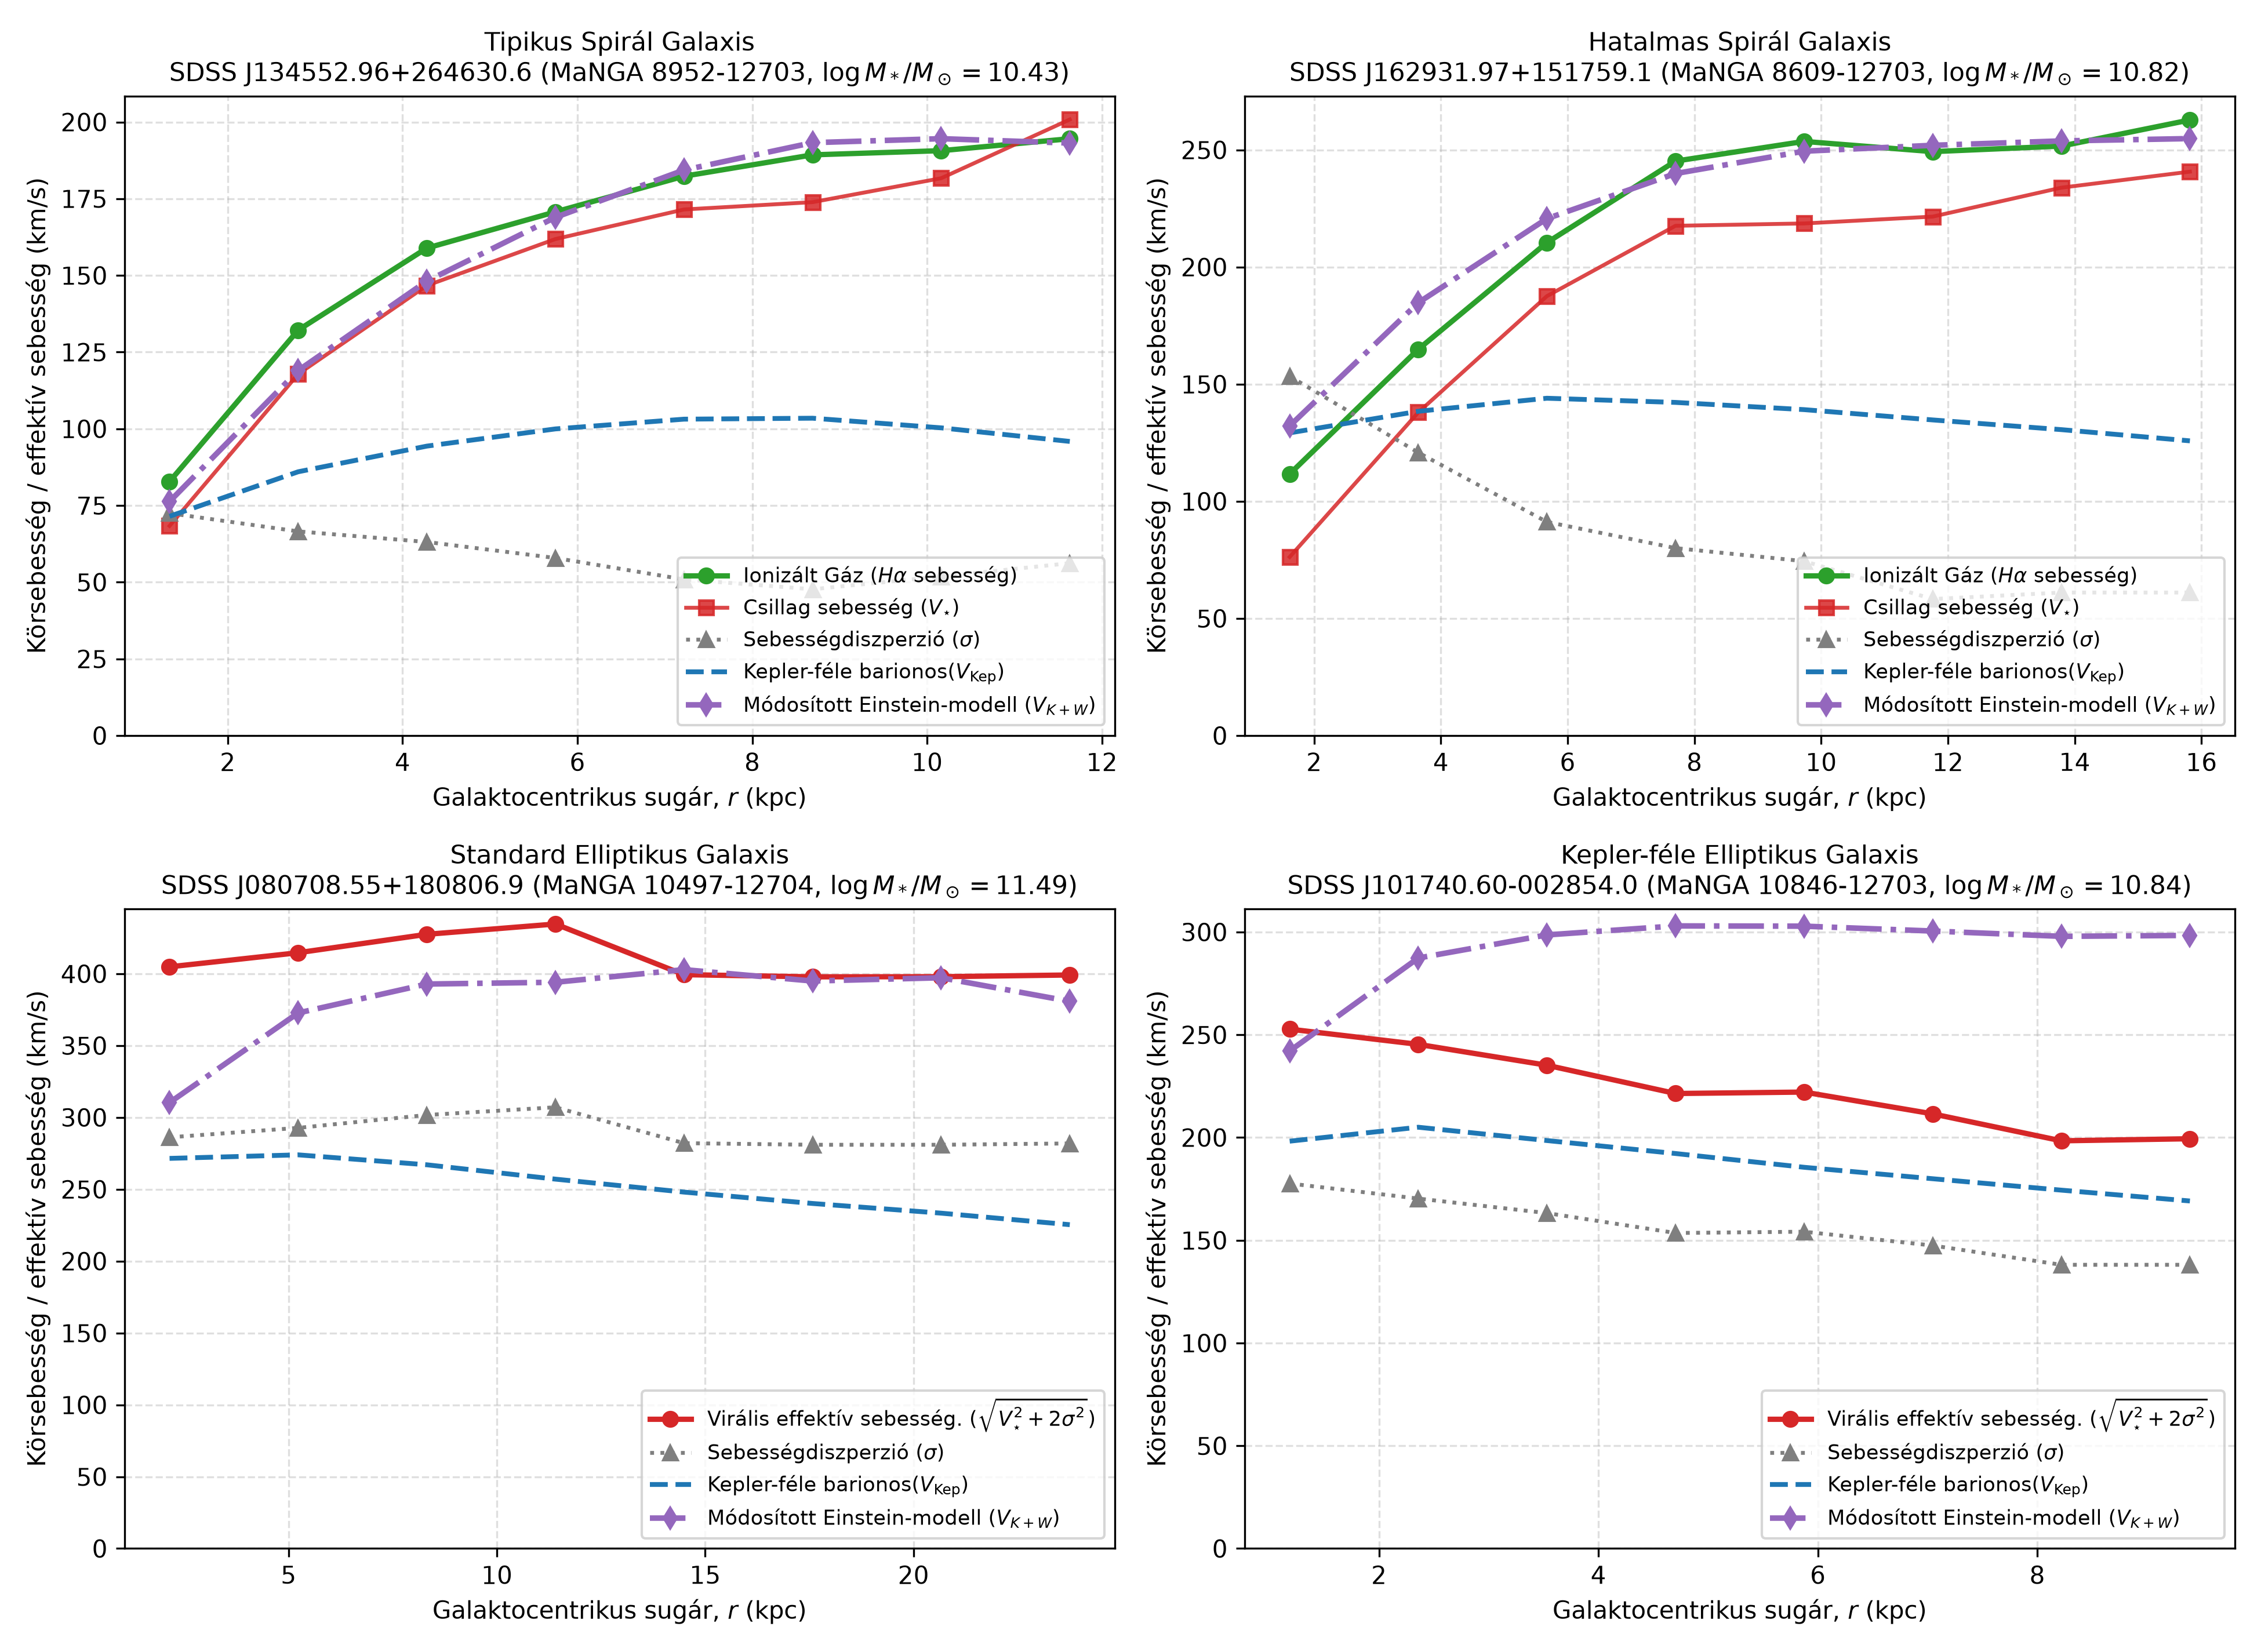
\includegraphics[width=0.95\textwidth]{case_studies_hu.png}
	\caption{Az SDSS MaNGA adatkészletből származó reprezentatív radiális kinematikai profilok, amelyek a megfigyelt gáz/csillag sebességeket összehasonlítják a Newton-Kepler-görbékkel és az Eq.~(\ref{eq:vel_profile}) egyenlet-előrejelzésekkel négy morfológiai és dinamikus tartományban.}
	\label{fig:case_studies}
\end{figure}

\section{Következtetések}

271 SDSS MaNGA galaxis vizsgálata megerősíti Tak\'acs (2026)~\cite{Takacs2026} egységes görbületfüggő mezőegyenleteit:
\begin{enumerate}
	\item \textbf{A sötétanyag-haló paramétereinek kiküszöbölése:} Egy univerzális csatolási pár ($\alpha_K = 0,800$, $\beta_W = 0,400$) használatával a modell spirális és elliptikus kinematikát reprodukál ($R = 0,8851$, nulla torzítás)~\cite{Takacs2026}.
	\item \textbf{A szükségtelenség nem kizáró ok:} Bár a megfelelő kalibráció szükségtelenné teszi a sötét anyag jelenlétét, ez még cáfolja, hogy ilyen tulajdonságú részecskék ne létezhetnének a téridő egzotikus örvényléseiként~\cite{Takacs2026b}.
	\item \textbf{Kozmikus és galaktikus léptékű konzisztencia:} A $\alpha_K / \beta_W = 2,0$ arány megegyezik a $\Lambda(K, C^2)$ operátorstruktúrával, ahol a $\alpha_K$ illeszkedik a késői idejű tágulási adatokhoz~\cite{Takacs2026,DESI2024}.
	\item \textbf{Maradékszórás:} A $\sim 15,2\%$ szóródás a modellezetlen HI gázfrakciókból, a por bizonytalanságaiból és az orbitális anizotrópiából ered.
\end{enumerate}

A jövőbeli felmérések (\textit{Euclid}, Rubin Obszervatórium) tovább fogják tesztelni a konform Weyl-nyíró tagot $\sqrt{C^2}$.

\section*{Köszönetnyilvánítás}

Az SDSS-IV MaNGA finanszírozását a Sloan Alapítvány, az Egyesült Államok Energiaügyi Minisztériuma és partnerei biztosították~\cite{Bundy2015}.
Köszönet a Google Gemini mesterséges intelligencia segítségének.

\begin{thebibliography}{9}
	
	\bibitem{Takacs2026} 
	Tak\'acs, F. (2026) A Version of Einstein's Equations Valid for the Entire Universe. \textit{International Journal of Astronomy and Astrophysics}, \textbf{16(3)}, 235--253. \\
	\url{https://doi.org/10.4236/ijaa.2026.163015}
	
	\bibitem{Takacs2026b} 
	Tak\'acs, F. (2026). ToE; Derivation of Quantum Phenomena from the Theory of Spacetime Geometry; Metric Tension in a Subatomic Environment.
	\textit{Journal of Modern Physics}, \textbf{17(10)}, 1245–1281.\\ \url{https://doi.org/10.4236/jmp.2026.1710055}

	\bibitem{DESI2024} 
	DESI Collaboration, Adame, A.G., Aguilar, J., Ahlen, S., et al. (2025) DESI 2024 VI: Cosmological Constraints from the Measurements of Baryon Acoustic Oscillations. \textit{Journal of Cosmology and Astroparticle Physics}, \textbf{2025}, 021. \\
	\url{https://doi.org/10.1088/1475-7516/2025/02/021}
	
	\bibitem{Rubin1980} 
	Rubin, V.C., Ford, W.K., Jr. and Thonnard, N. (1980) Rotational Properties of 21 Sc Galaxies with a Large Range of Luminosities and Radii, from NGC 4605 ($R = 4\text{ kpc}$) to UGC 2885 ($R = 122\text{ kpc}$). \textit{The Astrophysical Journal}, \textbf{238}, 471--487. \\
	\url{https://doi.org/10.1086/158003}
	
	\bibitem{Hamilton2008} 
	Hamilton, A.J.S. and Lisle, J.P. (2008) The River Model of Black Holes. \textit{American Journal of Physics}, \textbf{76}, 519--532. \\
	\url{https://doi.org/10.1119/1.2830526}
	
	\bibitem{Bundy2015} 
	Bundy, K., Bershady, M.A., Law, D.R., et al. (2014) Overview of the SDSS-IV MaNGA Survey: Mapping Nearby Galaxies at Apache Point Observatory. \textit{The Astrophysical Journal}, \textbf{798}, 7. \\
	\url{https://doi.org/10.1088/0004-637x/798/1/7}
	
	\bibitem{Romanowsky2003} 
	Romanowsky, A.J., Douglas, N.G., Arnaboldi, M., et al. (2003) A Dearth of Dark Matter in Ordinary Elliptical Galaxies. \textit{Science}, \textbf{301}, 1696--1698. \\
	\url{https://doi.org/10.1126/science.1087441}
	
\end{thebibliography}
\end{document}
